\documentclass{../notatki}

\title{Mechanika Ogólna}

\usetikzlibrary{calc}

\begin{document}

\tableofcontents

\setcounter{section}{-1}

\section{Wstęp}

\subsection{Całki}

Całki to operacje odwrotne do pochodnych. Dla funkcji $f(x)$ całka oznaczona
to pole pod wykresem funkcji $f(x)$ na przedziale $[a, b]$. Pozwalają nam
obliczyć pole pod krzywą, a także sumę nieskończenie wielu wartości funkcji.

\begin{figure*}[h]
  \centering
  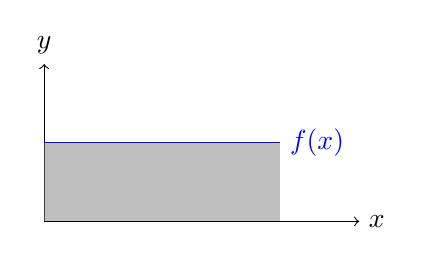
\begin{tikzpicture}
    \draw[->] (0, 0) -- (4, 0) node[right] {$x$};
    \draw[->] (0, 0) -- (0, 2) node[above] {$y$};
    \draw[domain=0:3, smooth, variable=\x, blue] plot
    ({\x}, {1}) node[right] {$f(x)$};
    \fill[fill=gray, fill opacity=0.5] (0, 0) -- (0, 1) -- (3, 1) --
    (3, 0) -- cycle;
  \end{tikzpicture}
\end{figure*}

$$
f(x) = 1, \quad \int_0^3 f(x) dx = \int_0^3 3 dx =\left[x\right]^3_0 = 3 - 0 = 3
$$
albo, o wiele prościej:

$$
\int_0^3 f(x) dx = 3 \cdot 1 = 3
$$
Naturalnie nie zawsze możemy obliczyć całkę oznaczoną w ten sposób. Wtedy
musimy posłużyć się bardziej zaawansowanymi metodami.

\section{Kinematyka}

Kinematyka to nauka o ruchu ciał.

\subsection{Wielkości średnie i chwilowe}

Wielkości średnie, to takie których doświadcza ciało w czasie $\Delta t$.
Z kolei wielkości chwilowe, to takie które opisują ciało w danym momencie.
Idealnym przykładem jest prędkość. $v(t)$ to prędkość chwilowa, a $v_{\Delta t}$
to prędkość średnia.

\subsection{Ruch}

Ruch ciała można opisać przy pomocy dwóch wielkości. Prędkości chwilowej ($v$),
oraz przyspieszenia chwilowego ($a$).

$$
v = \frac{\Delta s}{\Delta t}
$$

$$
v(t) = v_0 + a(t) \cdot t = v_0 + \int a(t) dt
$$

$$
a = \frac{\Delta v}{\Delta t} = v'
$$

Dla pozycji ciała $x$ mamy:

$$
x(t) = x_0 + v_0t + \frac{1}{2}a t^2
$$

$$
\Delta x = s = \int v(t) dt
$$

\subsection{Ruch w wielu wymiarach}

Aby opisać ruch w $n \in \mathbb{N}$ wymiarach, potrzebujemy po prostu $n$
wymiarowych wektorów. Dla ruchu w dwóch wymiarach mamy:

\begin{figure*}[h]
  \centering
  \begin{tikzpicture}
    \draw [->] (0,0) -- (4.0,0) node [below right] {$x$};
    \draw [->] (0,0) -- (0,4.0) node [above right] {$y$};
    \coordinate (A) at (0.5,1);
    \coordinate (B) at (3,3);
    \draw [->] (A) -- (B) node [midway, above] {$\vec{v}$};
    \draw [dashed] (A) -- (3,1) node [midway, below] {$\vec{v}_x$};
    \draw [dashed] (3,1) -- (3,3) node [midway, right] {$\vec{v}_y$};
    % draw the angle
    \draw[draw=blue] (A) ++(0:10mm) arc (0:39:10mm) node[midway,
    left]{$\alpha$};
  \end{tikzpicture}
\end{figure*}

$$
\vec{v}_x = |\vec{v}| \cos \alpha, \quad \vec{v}_y = |\vec{v}| \sin \alpha
$$

\subsection{Ruch po okręgu}

Dla ruchu po okręgu mamy:

$$
a = \frac{v^2}{r}
$$
Dla prędkości kątowej $\omega$ mamy:
$$
\omega = \frac{\Delta \phi}{\Delta t}
$$
gdzie $\phi$ to kąt ruchu po okręgu.

\section{Siły}

Miara wielkości oddziaływania ciał na siebie to siła.

$$
F = m \cdot a
$$
Dla siły grawitacyjnej działającej na ciało o masie $m$ pod kątem
$\alpha$ do osi $x$ mamy:

$$
F_g = m \cdot g \cdot \sin \alpha
$$

\subsection{Prawa Newtona}

\begin{enumerate}
  \item Ciało pozostaje w spoczynku lub porusza się ruchem jednostajnym
    prostoliniowym, jeżeli na nie nie działa żadna siła. $\sum F = 0
    \rightarrow \Delta v = 0$.
  \item Jeżeli na ciało działa siła, to ciało porusza się z przyspieszeniem
    proporcjonalnym do siły i odwrotnie proporcjonalnym do masy ciała.
  \item Jeżeli ciało działa na inne ciało siłą, to drugie ciało działa na
    pierwsze siłą o tej samej wartości, ale przeciwnie skierowaną.
\end{enumerate}

\subsection{Ciążenie powszechne}

Każda para ciał we wszechświecie oddziałuje na siebie siłą grawitacyjną.

$$
F_g = G \cdot \frac{m_1 \cdot m_2}{r^2}
$$
gdzie $G$ to stała grawitacyjna, $m_1$ i $m_2$ to masy ciał, a $r$ to odległość
między nimi.

\subsection{Tarcie}

Tarcie to siła przeciwna kierunku ruchu ciała. Wyróżniamy tarcie statyczne i
kinetyczne. Tarcie statyczne oddziałuje na ciała gdy te nie poruszają się, a
tarcie kinetyczne gdy ciała poruszają się. W pewnym sensie tarcie statyczne
określa siłę potrzebną do wzruszenia ciała, a tarcie kinetyczne to jaką siłę
trzeba utrzymać aby ciało poruszało się z daną prędkością.

\subsection{Popęd}

$$
J = F \cdot \Delta t
$$

\section{Energia}

Energia to miara zdolności ciała do wykonywania pracy. Energia kinetyczna to
energia którą ciało posiada dzięki swojemu ruchowi, a energia potencjalna to
energia którą ciało posiada dzięki swojemu stanowi.

$$
E_K = \frac{mV^2}{2}
$$

$$
W = E_{K1} - E_{K0} = \Delta E_K = F \cdot d = \int F(x) dx
$$

Wyróżniamy energie potencjalną grawitacyjną, związaną z wysokością ciała nad
pewnym ustalonym punktem.

$$
E_p = mgh
$$

Oraz energię potencjalną sprężystości sprężyny:

$$
E_p = \frac{1}{2}kd^2
$$
gdzie $k$ to stała sprężystości, a $d$ to odkształcenie sprężyny.

\subsection{Zasada zachowania energii}

W układzie izolowanym energia jest stała. Energia nie może zostać ani stworzona,
ani zniszczona.

$$
E_{t=0} = E_{t=t}
$$

\subsection{Tarcie i energia}

Praca siły tarcia jest zawsze ujemna, ponieważ działa ona przeciwnie do kierunku
ruchu ciała. Obecność tarcia powoduje, że energia kinetyczna ciała maleje.

\section{Dynamika układów wielu ciał}

Układy ciał to zbiory ciał, które oddziałują na siebie. Wewnątrz układu ciała
mogą oddziaływać na siebie siłami wewnętrznymi, a na zewnątrz siłami
zewnętrznymi. W układzie izolowanym suma sił wewnętrznych jest równa zeru.

\subsection{Środek masy}

Środek masy to punkt, w którym można zlokalizować całą masę układu. Jego
położenie w relacji do ciał w układzie może mieć wpływ na ruch układu.
Dla równej dystrybucji masy środek masy znajduje się w środku układu.
Np.: dla trójkąta środek masy znajduje się w punkcie przecięcia środkowych.

\begin{figure*}[h]
  \centering
  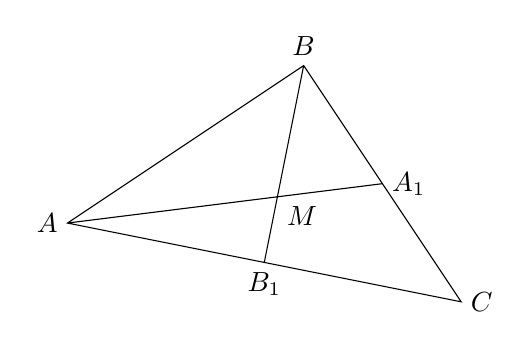
\begin{tikzpicture}
    \draw (0,1) coordinate[label=left:$A$] (A) --
    (3,3) coordinate[label=above:$B$] (B)  --
    (5,0) coordinate[label=right:$C$] (C) -- cycle
    (A) -- ($(B)!0.5!(C)$) coordinate[label=right:$A_1$](A1)
    (B)--($(A)!0.5!(C)$) coordinate[label=below:$B_1$](B1)
    (intersection cs:first line={(A)--(A1)},
    second line={(B)--(B1)}) coordinate[label=below right:$M$] (M);
  \end{tikzpicture}
\end{figure*}

Dla układu n ciał środek masy to będzie ważona średnia położeń ciał.

\subsection{Zasada zachowania pędu}

$$
p = m \cdot v
$$
W izolowanym układzie pęd jest stały.

$$
p_{t=0} = p_{t=t}
$$

\subsection{Zderzenia}

Zderzenia to procesy w których ciała zmieniają swoje prędkości. Rozróżniamy
zderzenia sprężyste, w których energia kinetyczna jest zachowana, oraz
niesprężyste, w których energia kinetyczna nie jest zachowana.

\section{Obroty}

\subsection{Bryła sztywna}

Bryła sztywna to ciało, które zachowuje swoją formę podczas ruchu.

\subsection{Przyspieszenie kątowe}

\begin{figure*}[h]
  \centering
  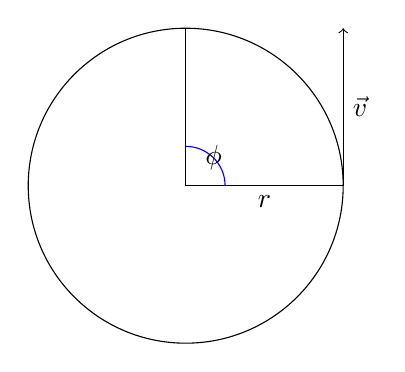
\begin{tikzpicture}
    \coordinate (O) at (0, 0);
    \coordinate (A) at (2, 0);
    \coordinate (A') at (0, 2);

    \draw (O) -- (A) node[midway, below] {$r$};
    \draw (O) -- (A');
    \draw[fill=none](0,0) circle (2.0);
    \draw[draw=blue] (O) ++(0:5mm) arc (0:90:5mm) node[midway]{$\phi$};
    \draw[->] (A) -- (2, 2) node[midway, right] {$\vec{v}$};

  \end{tikzpicture}
\end{figure*}

$$
\omega = \frac{\Delta \phi}{\Delta t}
$$

$$
\alpha = \frac{\Delta \omega}{\Delta t}
$$

$$
\int \alpha dt = \int d\omega
$$

$$
F_c = m \cdot a_c = m \cdot r \cdot \omega^2
$$
gdzie $a_c$ to przyspieszenie dośrodkowe, a $r$ to promień obrotu. Dla obiektu
o długości $l$ i jednorodnym rozłożeniu masy to $r = \frac{l}{2}$.

$$
\text{ rpm} = \frac{2\pi}{60} \text{ rad/s}
$$

\subsection{Bezwładność, pęd i energia}

$$
I = \sum m_i r_i^2
$$
czyli suma momentów bezwładności wszystkich punktów materialnych w ciele.
Moment bezwładności wyraża opór ciała na zmianę ruchu obrotowego.\\
Moment pędu:
$$
L = I \cdot \omega
$$
Moment siły:
$$
\tau = \frac{dL}{dt}
$$

\subsection{Moment bezwładności}

Moment obrotowy:
$$
\tau = I \cdot \alpha = I \cdot \frac{\Delta \omega}{\Delta t}
$$

$$
W = \frac{I\omega^2}{2}
$$

\subsection{Toczenie się}

Energia kinetyczna ruchu postępowego:
$$
E_K = \frac{mV^2}{2}
$$
Energia kinetyczna obrotu:
$$
E_K = \frac{I\omega^2}{2}
$$

\end{document}
